

\chapter{Local Optimality}
\label{sec:local-opt}

The first several \chaps\  have established the
fundamental definitions and constructions of this \paper.   This
\chap\ establishes the local optimality of the function
$\sigma:\op{DS}\to\ring{R}$ in a neighborhood of the decomposition
stars of the face-centered cubic and hexagonal close packings.

\section{Results}

Here is a sketch of the proof of local optimality.  The
face-centered cubic and hexagonal close packings score precisely
$8\,\pt$.  They also contain precisely eight tetrahedra around each
vertex.  In fact, the decomposition stars have $8$ quasi-regular
tetrahedra and $6$ other quad clusters.   The proof shows that each
of the $8$ quasi-regular tetrahedra scores at most $1\,\pt$.
Equality is obtained only when the tetrahedron is regular of side
$2$. Furthermore, the proof shows that each of $6$ quad clusters
have a nonpositive score.   It will follows from these facts that
any decomposition star with $8$ quasi-regular tetrahedra, $6$ quad
clusters, and no other standard clusters scores at most $8\,\pt$.
The case of equality is analyzed as well. The purpose of this \chap\
is to give a proof of the following theorem.

\begin{theorem} [Local Optimality] \label{lemma:local-optimality}
Let $D$ be a contravening decomposition star.  Let $U(D)$ be the
set of sphere packing vectors at distance at most $2t_0$ from the
origin.
%
 \index{UZ@$U(D)$}
 \index{local optimality}
Assume that
   \begin{enumerate}
      \item The set $U(D)$
         has twelve elements.
      \item There is a bijection $\psi$ between $U(D)$ and the kissing
         arrangement $U_{fcc}$ of twelve tangent unit balls in
         the face-centered cubic configuration, or a bijection
            with $U_{hcp}$ the twelve tangent unit balls in the
            hexagonal-close packing configuration;
            such that
            for all $v,w\in U(D)$, $|w-v|\le 2t_0$ if and only if
            $|\psi(w)-\psi(v)|=2$.  That is, the proximity
            graph of $U(D)$ is the same as the contact graph of
               $U_{fcc}$ or $U_{hcp}$.
   \end{enumerate}
Then $\sigma(D)\le 8\,\pt$.  Equality holds if and only if
   $U$ coincides with $U_{fcc}$ or $U_{hcp}$ up to a Euclidean
   motion.  Decomposition stars $D$ exist with $U(D)=U_{fcc}$ and
   others exist with $U(D) = U_{hcp}$.
\end{theorem}

\begin{remark}  This theorem is one of the key claims of
Section~\ref{sec:logic}.  This theorem is phrased slightly
differently from the Claim~\ref{claim-E} in
Section~\ref{sec:logic}. The reason for this is that we have not
formally introduced the plane graph $G(D)$ of a decomposition
star.  (This happens in Section~\ref{sec:stargraph}.)  Once $G(D)$
has been formally introduced, then
Theorem~\ref{lemma:local-optimality} can be expressed more
directly, as follows.  We let $G_{fcc}$ and $G_{hcp}$ be the plane
graphs attached to the decomposition stars of vertices in the
face-centered cubic and hexagonal-close packings, respectively.
(These graphs are independent of the vertices selected.)
\end{remark}

\begin{corollary}[Local Optimality - second version]
 \label{lemma:local-optimality2}
Contravening decomposition stars exist. If $D$ is a contravening
decomposition star, and if the plane graph of $D$ is isomorphic to
$G_{fcc}$ or $G_{hcp}$, then $\sigma(D) = 8\,\pt$.  Moreover, up
to Euclidean motion, $U(D)$ is the kissing arrangement of the $12$
balls around a central ball in the face-centered cubic packing or
the kissing arrangement of $12$ balls in the hexagonal-close
packing.
\end{corollary}

The following theorem is also one of the main results of this
\chap. It is a key part of the proof of local optimality.

\begin{theorem}\label{lemma:quad0} A quad cluster scores at most
$0$, and that only for a quad cluster whose corners have height
$2$, forming a square of side $2$. That is, $\sigma_R(D)\le 0$.
Other standard clusters have strictly negative scores:
$\sigma_R(D)<0$.
\end{theorem}\index{cluster!quad}

The argument that the score of a quad cluster is nonpositive is
general and can be used to prove that the score of any cluster
attached to a non-triangular standard region (as defined in
Definition~\ref{def:arc}) has nonpositive score.


\section{Rogers Simplices}

To prove Theorem~\ref{lemma:quad0}, we chop the cluster $(R,D)$
into small pieces and show that the ``density'' of each piece is
at most $\doct$. To prepare for this proof, this section describes
various small geometric solids that have a density at most
$\doct$.  The first of these is the Rogers simplex.

\begin{lemma} \label{lemma:rogers-lemma}
Let $R(a,b,c)$ be a Rogers simplex, with $1\le a < b < c$.  It has
a distinguished vertex (the terminal point of the edges of lengths
$a$, $b$, and $c$), which we assume to be the origin. Let
$A(a,b,c)$ be the volume of the intersection of $R(a,b,c)$ with a
ball of radius $1$ at the origin.  Then the ratio
    $$A(a,b,c)/\op{vol}(R(a,b,c))$$
is monotonically decreasing in each variable.\index{Rogers simplex}
\end{lemma}
\index{vertex!distinguished}
\begin{proof}
    This is Rogers's lemma, as formulated in \cite[Lemma~8.6]{part1}.
\end{proof}


\begin{lemma} \label{lemma:rogers-app} Consider the Rogers simplex $R(a,b,\sqrt2)$ with vertex
at the origin.  Assume $1\le a\le b$ and $\eta(2,2,2)\le
b\le\sqrt2$. Let $A$ be the volume of the intersection of the
simplex with a closed ball of radius $1$ at the origin. Then
    $$A\le \doct\,\op{vol}(R(a,b,\sqrt2)).$$
Equality is attained if and only if $a=1$ and $b=\eta(2,2,2)$ or for
a degenerate simplex of zero volume.
\end{lemma}\index{Rogers simplex}

\begin{proof} This is a special case of Lemma~\ref{lemma:rogers-lemma}. See the third
frame of Figure~\ref{fig:doct}.
\end{proof}

\begin{lemma} \label{lemma:wedge} Consider the wedge of a cone
    $$
    W =W(\alpha,z_0) =
    \{ t\, x : 0\le t \le 1, x\in P(\alpha,z_0)\}\subset\ring{R}^3,
    $$
where $P(\alpha,z_0)$ has the form
    $$
    P = \{(x_1,x_2,x_3) :
    x_3 = z_0,\   x_1^2+x_2^2+x_3^2\le 2,\ 0\le x_2\le \alpha x_1\},
    $$
with $z_0\ge1$.  Let $A$ be the volume of the intersection of the
wedge with $B(0,1)$. Then
    $$A\le\doct\,\op{vol}(W).$$
Equality is attained if and only if $W$ has zero volume.\index{cone}
\end{lemma}

\begin{proof} This is calculated in \cite[Sec. 4]{part2}.  See the
second frame of Figure~\ref{fig:doct}.
\end{proof}

\begin{lemma} \label{lemma:cone}
Let $C$ be the cone at the origin over a set $P$, where $P$ is
measurable and every point of $P$ has distance at least $1.18$
from the origin.  Let $A$ be the volume of the intersection of $C$
with $B(0,1)$. Then
    $$A\le\doct\,\op{vol}(C).$$
Equality is attained if and only if $C$ has zero volume.
\end{lemma}

\begin{proof} The ratio $A/\op{vol}(C)$ is at most $1/1.18^3 < \doct$.   See the
first frame of Figure~\ref{fig:doct}.
\end{proof}

\begin{figure}[htb]
  \centering
  \includegraphics{PS/haII42.ps}
  \caption{Some sets of low density.}
  \label{fig:doct}
\end{figure}

\section{Bounds on Simplices}\label{sec:bounds-simplex}

In this and future \chaps,
we rely on some inequalities that are not proved in
this paper.  There is an archive of hundreds of inequalities that
have been proved by computer.  This full archive appears in
\cite{web}.  The justification of these inequalities appears in
the same archive.  (The proofs of these inequalities were executed
by computer.)  An explanation of how computers are able to prove
inequalities can be found in \cite{algorithm} and \cite{part1}.
Each inequality carries a nine-digit identifying number. To invoke
an inequality, we state it precisely, and give its identifying
number, e.g. \calc{123456789}. The first of these appears in Lemma
\ref{lemma:1pt}.  Some results rely on a simple combination of
inequalities, rather than a single inequality.  To make it easier
to reference a group of inequalities, the archive at \cite{web}
gives a separate nine-digit identifier to certain groups of
inequalities.  This permits us to reference such a group by a
single number.
%
 \index{calc@\calc{123456789}}


\begin{definition} \label{def:point}
Recall that the constant $\pt$, a {\it point},  is equal to
$\sigma(S)$, where $S$ is a regular tetrahedron with edges of
length $2$. We have $\pt = 4\arctan(\sqr2/5) - \pi/3 \approx
0.05537$.
\end{definition}\index{point}


\begin{lemma} \label{lemma:1pt}
%\proclaim{Lemma 3.13}
A quasi-regular tetrahedron $S$ satisfies $\sigma(S)\le 1\,\pt$.
Equality occurs if and only if the quasi-regular tetrahedron is
regular of edge length $2$.\index{quasi-regular!tetrahedron}
%
\end{lemma}

\begin{proof}
This is \calc{586468779}.
\end{proof}

\begin{remark}  The reader who wishes to dig more deeply into this particular
proof may do so.   An early published proof of this lemma was not
fully automated (see \cite[Lemma~9.1.1]{part1}).  This early proof
show by conventional means that $\sigma(S)\le 1\,\pt$ in an
explicit neighborhood of $(2,2,2,2,2,2)$.
\end{remark}

\begin{lemma} \label{lemma:quarter0}
A quarter in the $Q$-system scores at most $0$. That is,
$\sigma(Q)\le 0$. Equality is attained if and only if five edges
have length $2$ and the diagonal has length $\sqrt8$.\index{quarter}
\end{lemma}

\begin{proof}  Throughout the proof of this lemma, we will refer to
quarters with five edges of length $2$ and one of length $\sqrt8$
as {\it extremal}\index{extremal (quarter)} quarters.  We make use
of the definition of $\sigma$ on quarters from
Definition~\ref{def:sigma}. The general context (that is, contexts
other than $(2,1)$ and $(4,0)$) of upright quarters is established
by the inequalities\footnote{\calc{522528841} and
\calc{892806084}} that hold for all upright quarters $Q$ with
distinguished vertex $v$:
    $$
    \begin{array}{lll}
    &2\Gamma(Q) + \svor_0(Q,v) - \svor_0(Q,\hat v) \le 0\\
    &\svor(Q,v) + \svor(Q,\hat v) +\svor_0(Q,v) - \svor_0(Q,\hat v)\le0.
    \end{array}
    $$
Equality is attained if and only if the quarter is extremal.
%Calculations~\ref{calc:3.13.3} and \ref{calc:3.13.4}.
For the remaining quarters (that is contexts $(2,1)$ and $(4,0)$),
it is enough to show that $\Gamma(Q)\le0$, if $\eta^+\le\sqrt2$
and $\svor(Q,v)\le0$, if $\eta^+\ge\sqrt2$.

Consider the case $\eta^+\le\sqrt2$.  If $Q$ is a quarter such that
every face has circumradius at most $\sqrt2$,
then\footnote{\calc{346093004}} $\Gamma(Q)\le0$.  Equality is
attained if and only if the quarter is extremal.
% from Calculation~\ref{calc:small-simplex}.
Because of this, we may assume that the circumradius of $Q$ is
greater than $\sqr2$. The inequality $\eta^+(Q)\le\sqr2$ implies
that the faces of $Q$ along the diagonal have nonnegative
orientation. The other two faces have positive orientation, by
Lemma~\ref{lemma:neg-orient-tet}. Since
(Definition~\ref{def:svor})
    $$4\Gamma(Q)=\sum_{i=1}^4 \svor(Q,v_i),$$
it is enough to show that $\svor(Q)<0$.  Since the orientation of
every face is nonnegative and the circumradius is greater than
$\sqrt2$, $\svor(Q,\sqrt2)$ is a strict truncation of the $V$-cell
in $Q$, so that
    $$\svor(Q)<\svor(Q,\sqrt2).$$
We show the right hand side is nonpositive.  Let $v$ be the
distinguished vertex of $Q$.  Let $A$ be $1/3$ the solid angle of
$Q$ at $v$ . By the definition of $\svor(Q,\sqrt2)$, it is
nonpositive if and only if
    \begin{equation}
        A\le \doct \,\op{vol}(\op{VC}(Q,v)\cap B(v,\sqrt2)).
        \label{eqn:Adoct}
    \end{equation}
($\op{VC}(Q,0)$ is defined in Section~\ref{sec:rules}.) The
intersection $\op{VC}(Q,v)\cap B(v,\sqrt2)$ consists of $6$ Rogers
simplices $R(a,b,\sqrt2)$, three conic wedges (extending out to
$\sqrt2$), and the intersection of $B(v,\sqrt2)$ with a cone over
$v$. By Lemmas~\ref{lemma:rogers-app}, \ref{lemma:wedge}, and
\ref{lemma:cone}, these three types of solids give inequalities
like that of Equation~\ref{eqn:Adoct}. Summing the inequalities
from these Lemmas, we get Equation~\ref{eqn:Adoct}.

Consider the case $\eta^+\ge\sqrt2$ and $\sigma=\svor$. If the
quarter is upright, then\footnote{\calc{40003553}} $\svor(Q)\le0$.
The quarters achieving equality are extremal.
%the result follows from Calculation~\ref{calc:3.13.2}.
Thus, we may assume the quarter is flat.  If the orientation of a
flat quarter is negative along the face containing the origin and
the diagonal, then\footnote{\calc{5901405}} $\svor(Q)\le0$. The
quarters achieving equality are extremal.
%Calculation~\ref{calc:3.13.1}.
In the remaining case, the only possible face along which the
orientation is negative is the top face.  This means that the
analytic continuation defining $\svor(Q)$ is the same as
    $$4(-\doct\op{vol}(X) + \sol(X)/3),$$
where $X$ is the subset of the cone at $v$ over $Q$ consisting of
points in that cone closer to $v$ than to any other vertex of $Q$.
The extreme point of $X$ has distance at least $\sqrt2$ from $v$
(since $\eta^+$ and hence the circumradius of $Q$ are at least
$\sqrt2$).  Thus,
    $$\svor(Q) \le \svor(Q,\sqrt2).$$
We have $\svor(Q,\sqrt2)\le0$ as in the previous paragraph, by
Lemma~\ref{lemma:rogers-app}, \ref{lemma:wedge}, and
\ref{lemma:cone}. If equality is attained, the wedges and cones
must have zero volume, and each Rogers simplex must have the form
$R(1,\eta(2,2,2),\sqrt2)$ (or zero volume). This happens exactly
when the flat quarter has five edges of length $2$ and a diagonal
of length $\sqrt8$.  This completes the proof. \end{proof}

\begin{lemma} \label{lemma:simplex0}
Let $S$ be a simplex all of whose faces have circumradius at most
$\sqrt2$.  Assume that $S$ is not a quasi-regular tetrahedron or
quarter.  Then $\svor(S)<0$.
\end{lemma}

\begin{proof} The assumptions imply that the orientation is positive
along each face.  Let $v$ be the distinguished vertex of $S$.

Assume first that there are at least $2$ edges of length at least
$2t_0$ at the origin or that there are two opposite edges of length
at least $2t_0$.  Then the circumradius $b$ of each of the three
faces at $v$ is at least $\eta(2,2t_0,2) > 1.207$.  By the
monotonicity properties of the circumradius of $S$, the simplex $S$
has circumradius at least that of the simplex $S(2,2,2,2,2,2t_0)$,
which a calculation shows is greater than $1.3045$.  By definition,
$\svor(S)<0$ if and only if
    $$
    \sol(|S|\cap B(v,1))/3 < \doct \op{vol}(\op{VC}(S,0)).
    $$
This inequality breaks into six separate inequalities
corresponding to the six Rogers's simplices $R(a,b,c)$
constituting $\op{VC}(S,0)$. Rogers's
Lemma~\ref{lemma:rogers-lemma} shows each of the six Rogers's
simplices has density at most that of $R(1,1.207,1.3045)$, which
is less than $\doct$.  The result follows in this case.

Now assume that there is at most $1$ edge of length at least
$2t_0$ at the origin, and that there is not a pair of opposite
edges of length at most $2t_0$.  There are four cases up to
symmetry, depending on which edges have length at least $2t_0$,
and which have shorter length.  Let $S$ be a simplex such that
every face has circumradius at most $\sqrt2$.  We
have\footnote{\calc{629256313}, \calc{917032944},
\calc{738318844}, and \calc{587618947}}
$\svor(S(y_1,y_2,\ldots,y_6))<0$ for $(y_1,\ldots,y_6)$ in any of
the following four domains:
    $$
    \begin{array}{lll}
        \ [2t_0,\sqrt8][2,2t_0]^3[2t_0,\sqrt8][2,2t_0], &
        \ [2t_0,\sqrt8][2,2t_0]^3[2t_0,\sqrt8]^2,\\
        \ [2,2t_0]^3[2t_0,\sqrt8]^2[2,2t_0],&
        \ [2,2t_0]^3[2t_0,\sqrt8]^3
    \end{array}
    $$
\end{proof}

\bigskip
\section{Breaking Clusters into Pieces}
\label{sec:break_piece}

As we stated above, the strategy in the proof of local optimality
will be to break quad clusters into smaller pieces and then show
that each piece has density at most $\doct$.  There are several
preliminary lemmas that will be used to prove that this
decomposition into smaller pieces is well-defined.  These lemmas
are presented in this section.


\begin{lemma} \label{lemma:no-eta-barrier}
Let $T$ be a triangle whose circumradius is less than $\sqrt2$.
Assume that none of its edges passes through a barrier in $\CalB$.
Then $T$ does not overlap any barrier in $\CalB$.\index{triangle}
\end{lemma}

\begin{proof}  By hypothesis no edge of $T$ passes through an edge in
the barrier.  By Lemma~\ref{lemma:no-pass-sqrt2}, no edge of a
barrier passes through $T$. Hence they do not overlap.
\end{proof}

\begin{lemma} \label{lemma:eta-barrier}
Let $T=\{u,v,w\}$ be a set of three vertices whose circumradius is
less than $\sqrt2$.  Assume that one of its edges $\{v,w\}$ passes
through a barrier $b=\{v_1,v_2,v_3\}$ in $\CalB$.  Then
    \begin{itemize}
        \item The edge $\{v,w\}$ has length between $2t_0$ and $\sqrt8$.
        \item The vertex $u$ is a vertex of $b$.
        \item One of the endpoints $y\in\{v,w\}$ is such that
            $\{y,v_1,v_2,v_3\}$ is a simplex in $\CalQ$.
    \end{itemize}
\end{lemma}

\begin{proof}
    The edge $\{v,w\}$ must have length at least $2t_0$ by
Lemma~\ref{lemma:2t0-doesnt-pass-through}. If the edge $\{u,v\}$
has length at least $2t_0$, it cannot pass through $b$ because of
Lemma~\ref{lemma:single-enclosed}.  If it has length at most
$2t_0$, it cannot pass through $b$ because of
Lemma~\ref{lemma:2t0-doesnt-pass-through}. Hence $\{u,v\}$ and
similarly $\{u,w\}$ do not pass through $b$.  The edges of $b$ do
not pass through $T$.  The only remaining possibility is for $u$
to be a vertex of $b$.

If $b$ is a quasi-regular triangle,
Lemma~\ref{lemma:qrtet-pair-pass} gives the result. If $b$ is a
face of a quarter in the $Q$-system, then
Lemma~\ref{lemma:pass-makes-quarter} gives the result.
\end{proof}

\begin{definition} [Law of Cosines]
\index{arc}\index{law of cosines}  Consider a triangle with sides
$a$, $b$, and $c$.  The angle opposite the edge of length $c$ is
given as
    $$
    \begin{array}{lll}
    \arc(a,b,c)&=\arccos((a^2+b^2-c^2)/(2a b))= \frac{\pi}2 +
      \arctan{\frac {c^2-a^2-b^2}{\sqrt{u(a^2,b^2,c^2)}}}\\
      &\quad\text{with } u(x,y,z) = -x^2-y^2-z^2+2 x y + 2 y z + 2
      z x.
    \end{array}
    $$
\end{definition}

\begin{lemma}[First separation lemma]\label{lemma:sqrt2-cone-avoidance}
    Let $v$ be a vertex of height at most $\sqrt8$.  Let $v_2$ and
    $v_3$ be such that
    \begin{itemize}
        \item $0$, $v$, $v_2$, and $v_3$ are distinct vertices,
        %\item $\{0,v,v_2,v_3\}\not\in \CalQ_0$, and
        \item $\eta(0,v_2,v_3)<\sqrt2$.
    \end{itemize}
    Then the open cone at the origin over the set $B(0,\sqrt2)\cap
     B(v,\sqrt2)$ does not meet the closed cone $C$ at the origin over
     the convex hull of $\{v_2,v_3\}$.
\end{lemma}

\begin{proof}
Let $D$ be the open disk spanning the circle of intersection of
$B(0,\sqrt2)$ and $B(v,\sqrt2)$.  It is enough to show that this
disk does not meet $C$.  This disk is contained in $B(v,\sqrt2)$,
so we bound this ball away from the given cone.

Assume for a contradiction that these two sets meet.  Let $v'$ be
the reflection of $v$ through the plane $P = \{0,v_2,v_3\}$.

If the closest point $p$ in $P$ to $v$ lies outside $C$, then the
edge constraints $|v|\le\sqrt8$ forces the closest point in $C$ to
lie along the edge $\{0,v_2\}$ or $\{0,v_3\}$.  Since
$|v_2|,|v_3|\le\sqrt8$, this closest point has distance at least
$\sqrt2$ from $v$. Thus, we may assume that the closest point in
$P$ to $v$ lies in $C$.

Assume next that the closest point in $P$ to $v$ lies in the
convex hull of $0$, $v_2$, and $v_3$.  We obtain an edge
$\{v,v'\}$ of length at most $\sqrt8$ that passes through a
triangle of circumradius less than $\sqrt2$. This contradicts
Lemma \ref{lemma:no-pass-sqrt2}.

Assume finally that the closest point lies in the cone over
$\{v_2,v_3\}$ but not in the convex hull of $0$, $v_2$, $v_3$. By
moving $v$ toward $C$ (preserving $|v|$), we may assume that
$|v-v_2|=|v-v_3|=2$.  Stretching the edge $\{v_2,v_3\}$, we may
assume that the circumradius of $\{0,v_2,v_3\}$ is precisely
$\sqrt2$.  Since the closest point in $P$ is not in the convex
hull of $\{0,v_2,v_3\}$, we may move $v_2$ and $v_3$ away from $v$
while preserving the circumradius and increasing the lengths
$|v-v_2|$ and $|v-v_3|$.  By moving $v$ again toward $C$, we may
assume without loss of generality that $|v_2|=|v_3|=2$ and
$|v_2-v_3|=\sqrt8$. We have reduced to a one-parameter family of
arrangements, parameterized by $|v|$. We observe that the disk in
the statement of the lemma is tangent to the segment $\{v_2,v_3\}$
at its midpoint, no matter what the value of $|v|$ is.  Thus, in
the extremal case, the open disk does not intersect the segment
$\{v_2,v_3\}$ or the cone $C$ that it generates.  This completes
the proof.
\end{proof}

\begin{lemma}[Second separation lemma]\label{lemma:cone-avoidance}
     Let $v_1$ be a vertex of height at most $2t_0$.  Let $v_2$
     and
     $v_3$ be such that
     \begin{itemize}
        \item $0$, $v_1$, $v_2$, and $v_3$ are distinct vertices,
        \item $\{0,v_1,v_2,v_3\}\not\in \CalQ_0$, and
        \item $\{0,v_2,v_3\}$ is a barrier.
     \end{itemize}
     Then the open cone at the origin over the set $B(0,\sqrt2)\cap
     B(v_1,\sqrt2)$ does not meet the closed cone $C$ at the origin over $\{v_2,v_3\}$.
\end{lemma}

\begin{proof}
Since $v_1$ has height at most $2t_0$, and $\{0,v_2,v_3\}$ is a
barrier, it follows from Lemma~\ref{lemma:diags-engulf} that
$\{0,v_1,v_2,v_3\}$ is in the $Q$-system if $|v_1-v_2|\le 2t_0$
and $|v_1-v_3|\le 2t_0$.  This is contrary to hypothesis. Thus, we
may assume without loss of generality that $|v_1-v_2|>2t_0$.

By arguing as in the proof of
Lemma~\ref{lemma:sqrt2-cone-avoidance}, we may assume that the
orthogonal projection of $v_1$ to the plane $P$ is a point in the
cone $C$. Let $v_1'$ be the reflection of $v_1$ through $C$.  We
have that either $\{v_2,v_3\}$ passes through $\{0,v_1,v'_1\}$ or
$\{v_1,v'_1\}$ passes through $\{0,v_2,v_3\}$.  We may assume for
a contradiction that $|v_1-v'_1|<\sqrt8$.

If $\{v_2,v_3\}$ passes through $\{0,v_1,v'_1\}$, then $v_2$ and
$v_3$ are anchors of the diagonal $\{v_1,v'_1\}$ by
Lemma~\ref{lemma:pass-anchor}.  This gives the contradiction
$|v_1-v_2|\le2t_0$.

If $\{v_1,v'_1\}$ passes through $\{0,v_2,v_3\}$, then by
Lemma~\ref{lemma:qrtet-pair-pass} $\{0,v_2,v_3\}$ is a face of a
quarter. Moreover, $v_1$ and $v'_1$ are anchors of the diagonal of
that quarter by Lemma~\ref{lemma:pass-anchor}.  Since
$|v_1-v_2|>2t_0$, then diagonal must not have $v_2$ as an
endpoint, so that the diagonal is $\{0,v_3\}$.
Lemma~\ref{lemma:pass-makes-quarter} forces one of $|v_1-v_2|$ or
$|v_1'-v_2|$ to be at most $2t_0$. But these are both equal to
$|v_1-v_2|>2t_0$, a contradiction.
\end{proof}


\begin{definition}  We define an enlarged set of simplices
$\CalQ_0'$.  Let $\CalQ_0'$ be the set of simplices $S$ with a
vertex at the origin such that either $S\in\CalQ_0$, or $S$ is a
simplex with a vertex at the origin and with circumradius less
than $\sqrt2$ such that none of its edges passes through a
barrier.\index{Q@$\CalQ_0'$}
\end{definition}

\begin{lemma}  The simplices in $\CalQ_0'$ do not overlap one another.
\end{lemma}

\begin{proof}
The simplices in $\CalQ_0$ are in the $Q$-system and do not
overlap.  No edge of length less than $\sqrt8$ passes through any
edge of a simplex in $\CalQ_0'\setminus \CalQ_0$, by
Lemma~\ref{lemma:no-pass-sqrt2}.  By construction, none of the
edges of a simplex in $\CalQ_0'\setminus\CalQ_0$ can passes
through a barrier, and this includes all the faces of $\CalQ_0$.
Thus, there is no overlap.
\end{proof}

\begin{definition}
\label{def:C'}
Let $v$ be a vertex of height at most $2.36=2(1.18)$.  Let $C(v)$
be the cone at the origin generated by the intersection
$B(v,\sqrt2)\cap B(0,\sqrt2)$.  Define a subset $C'(v)$ of $C(v)$
by the conditions.
   \begin{enumerate}
   \item $x\in C(v)$.
   \item $x$ is closer to $0$ than to $v$.
   \item $x\in B(0,\sqrt2)$.
   \item $x$ does not lie in the cone over any simplex in
   $\CalQ_0$.
   \item For every vertex $u\ne0,v$ such
   that the face $\{0,u,v\}$ is a barrier or
   has circumradius less than $\sqrt2$
   and such that
   none of the edges of this face pass through a barrier, we have
   that $x$ and $v$ lie in the same half-space bounded by the
   plane perpendicular to $\{0,u,v\}$ and passing through $0$ and
   the circumcenter of $\{0,u,v\}$.
   \item For every simplex $\{0,v_1,v_2,v\}\in \CalQ_0$, the segment
   $\{x,v\}$ does not cross through the cone $C(\{0,v_1,v_2\})$.
   \end{enumerate}
\index{C'@$C'(v)$}
\end{definition}

\begin{lemma}\label{lemma:C'}
For every vertex $v$ of height at most $2.36$, we have
$C'(v)\subset \op{VC}(0)$.
\end{lemma}


% Assume that $x$ satisfies the following
%conditions
%   \begin{enumerate}
%   \item $x$ is closer to $0$ than to $v$.
%   \item $x\in B(0,\sqrt2)$.
%   \item $x$ does not lie in the cone over any simplex in
%   $\CalQ_0$.
%   \item $x\in\op{VC}(u)$ for some $u\ne 0,v$.
%   \end{enumerate}
%Then one of the following two conditions hold.
%   \begin{enumerate}
%   \item There is a vertex $u_1\ne0,v$ such
%   that the face $\{0,u_1,v\}$ is a barrier or
%   has circumradius less than $\sqrt2$;
%   none of the edges of this face pass through a barrier; and $x$
%   is closer to $u_1$ than to $0$.
%   \item There exists $\{0,v_1,v_2,v\}\in \CalQ_0$ such that the
%   conditions of the decoupling lemma hold
%   (Lemma~\ref{lemma:V-cell-local}).  That is, $x$ is closer to
%   the origin than to both $v_1$ and $v_2$ and the segment
%   $\{x,v\}$ crosses through the cone $C(\{0,v_1,v_2\})$.
%   \end{enumerate}
%\end{lemma}

\begin{proof}
Assume for a contradiction that $x\in C'(v)\cap \op{VC}(u)$, with
$u\ne 0$. Lemma~\ref{lemma:sqrt2-unobstructed} implies that $x$ is
unobstructed at $0$.  Thus $|x-u|<|x|\le\sqrt2$.

Assume that the hypotheses of Condition~5 in Definition~\ref{def:C'} are
satisfied.
This, together
with $x\in C(v)$ implies that $\eta(\{0,u,v\})<\sqrt2$. An element
$x$ that is closer to $0$ than to $v$ and in the same half-space
as $v$ (in the half-space bounded by the perpendicular plane to
$\{0,u,v\}$ through $0$ and the circumcenter of $\{0,u,v\}$) is
closer to $0$ than to $u$, which is contrary to $x\in\op{VC}(u)$.
This completes the proof, except in the case that an edge of the
triangle $\{0,u,v\}$ passes through a barrier $b$. Assume that
this is so.

The edge $\{0,v\}$ cannot pass through a barrier because it is too
short (length less than $2t_0$).

Suppose that the edge $\{u,v\}$ passes through a barrier $b$.  By
Lemma~\ref{lemma:eta-barrier} applied to $T=\{0,u,v\}$, the origin
is  a vertex of $b$.  There are three possibilities
   \begin{enumerate}
   \item $x$ is obstructed from $u$ by $b$.
   \item $x$ is obstructed from $v$ by $b$.
   \item $x$ is not obstructed from either $u$ or $v$ by $b$.
   \end{enumerate}
The first possibility runs contrary to the hypothesis
$x\in\op{VC}(u)$.
%In the second possibility, $x$ has distance at
%least $\sqrt2$ from both $u$ and $v$, which is contrary to the
%derived inequalities $|x-u|<|x|\le\sqrt2$.
The second possibility, together with
Lemma~\ref{lemma:cone-avoidance}, implies that $\{v,b\}$ is a
simplex in the $Q$-system. This is contrary to Condition 6
defining $C'(v)$.
% so that none of the edges of $\{v,0,v_1\}$ or
%$\{v,0,v_2\}$ pass through a barrier. If $x$ is closer to $v_1$
%(or $v_2$) than $0$, then the desired conclusion holds with
%$u_1=v_1$ (or $u_1=v_2$). Otherwise the conditions of the
%decoupling lemma hold.

The third possibility is eliminated as follows.
Every point in the half-space containing $v$ and bounded by the plane
of $b$
 \begin{itemize}
 \item is obstructed at $u$ by $b$, or
 \item has distance at least $\sqrt2$ from $u$ (because each edge of
 $b$ has this property).
 \end{itemize}
Since $x$ has neither of these properties, we find that $x$
 must
lie in the same half space bounded by the plane of $b$ as $u$. Let
$S$ be the simplex formed by $b$ and $v$.  If $S\not\in \CalQ_0$,
then Lemma~\ref{lemma:cone-avoidance} shows that no part of the
cone $C(v)$ lies in the same half space as $u$.  So $S\in
\CalQ_0$.  By Condition~6 on $C'(v)$, the line from $x$ to $v$
does not intersect the cone at the origin over $b$.  But then the
arc-length of the geodesic on the unit sphere running from the
projection of $x$ to the projection of $v$ is at least
$\op{arc}(|v|,\sqrt8,2)\ge \op{arc}(|v|,\sqrt2,\sqrt2)$. This
measurement shows that $x$ lies outside the cone $C(v)$, which is
contrary to assumption.

Suppose that the edge $\{0,u\}$ passes through the barrier $b$. By
Lemma~\ref{lemma:eta-barrier} applied to $T=\{0,u,v\}$, we get
that $v$ is a vertex of $b$.   There are again three possibilities
   \begin{enumerate}
   \item $x$ is obstructed from $u$ by $b$.
   \item $x$ is not obstructed from either $u$ or $0$ by $b$.
   \item $x$ is obstructed from $0$ by $b$.
   \end{enumerate}
The first possibility runs contrary to the hypothesis $x\in
\op{VC}(u)$.  The second places $x$ outside the convex hull of
$0$, $b$, $u$ and gives $|x-u|+|x|>\sqrt8$, which is contrary to
$|x-u|\le|x|\le\sqrt2$. The third possibility cannot occur by the
observation made at the beginning of the proof that $x$ is
unobstructed at $0$.
\end{proof}

It follows from the definition that $C'(v)$ is star convex at the
origin. We make this more explicit in the following lemma.

\begin{lemma}\label{lemma:F'}
Assume $|v|\le 2.36$.  Let $F(v)$ be the intersection of
$\Omega(0)\cap\Omega(v)$; that is, the face of the Voronoi cell of
$\Omega(0)$ associated with the vertex $v$.  Let $F'(v)$ be the
part of $F(v)\cap B(0,1.18)$ that is not in the cone over any
simplex in $\CalQ_0$. Let $H(v)$ be the closure
of the union of segments from
the origin to points of $F'(v)$.
Let $C''(v)$ be the cone at the origin spanned
by $B(0,1.18)\cap B(v,1.18)$. Then the closure of $C'(v)\cap C''(v)$
is equal to  $H(v)$.
\end{lemma}

\begin{proof} We have $F'(v)\subset C''(v)$.

First we show that $F'(v)$ lies in the closure of $C'(v)$.  For
this, we check that points of $F'(v)$ satisfy the (closed
counterparts of) Conditions 1--6 defining $C'(v)$
(see Definition~\ref{def:C'}). Conditions 1--4
are immediate from the definitions.  If $u$ is a vertex as in
Condition 5, then the half-space it determines is that containing
the origin and the edge of the Voronoi cell determined by $u$ and
$v$.  Condition 5 now follows.  Consider Condition 6.  Suppose
that $\{x,v\}$ crosses the cone $\{0,v_1,v_2\}$ and that $x\in
F'(v)$.
(The point of intersection has height  at most $\sqrt2$ and
hence lies in the convex hull of $\{0,v_1,v_2\}$.)
This implies that $x$ is obstructed at $v$.  By
Lemma~\ref{lemma:unobstr-t0}, this implies that $|x-v|\ge t_0$.
Since $x$ is equidistant from $v$ and the origin, we find that
$|x|\ge t_0$, which is contrary to $x\in B(0,1.18)$.

To finish the proof, we show that $C'(v)\cap C''(v)\subset H(v)$.
For a contradiction, consider a point $x\in C'(v)\cap C''(v)$ that is
not in $H(v)$.  It must lie in the cone over some other face of
the Voronoi cell; say that of $u$. The constraints force the
circumradius of $T=\{0,v,u\}$ to be at most $1.18$.  The edges of
$T$ are too short to pass through a barrier.  Thus, Condition 5
defining $C'(v)$ places a bounding plane that is perpendicular to
$T$ and that runs through the origin and the circumcenter of $T$.
This prevents $x$ from lying in the cone over the face of the
Voronoi cell attached to $u$.
\end{proof}

\begin{remark} In the lemma,
it is enough to consider simplices along $\{0,w\}$, because
$$
  \arc(|v|,\sqrt8,2) > \arc(|v|,1.18,1.18).
$$
\end{remark}

\begin{corollary}\label{lemma:all-in-C'}
If $x\in \op{VC}(0)$, with $0< |x|\le1.18$,  if the point at distance
$1.18$ from $0$ along the ray $(0,x)$ does not lie in
$\op{VC}(0)$, and if $x$ is not in the cone over any simplex of
$\CalQ_0$, then there is some $v$ such that $x\in C'(v)$, and
$|v|\le 2.36$.
\end{corollary}

\begin{proof} If $x\in \op{VC}(0)\cap B(0,1.18)$,
then $x\in \Omega(0)\cap B(0,1.18)$ by Lemma~\ref{lemma:VC-Omega}.
$x$ lies in the cone over some face $F(v)$ of the Voronoi cell
$\Omega(0)$. The hypotheses imply that $x$ lies in the cone over
$F'(v)$. Lemma~\ref{lemma:F'} implies that $x\in C'(v)$.
\end{proof}

\begin{lemma}
Assume that $|u|\le 2.36$ and that $|v|\le 2.36$.   The sets
$C'(u)$, $C'(v)$ do not overlap for $u\ne v$.
\end{lemma}

\begin{proof}  If there is some $x$ in the overlap,
then the circumradius of $\{0,u,v\}$ is less than $\sqrt2$. If no
edge of $\{0,u,v\}$ passes through a barrier, then the defining
conditions of $C'(u)$ and $C'(v)$ separate them along the plane
perpendicular to $\{0,u,v\}$ and passing through the origin and
the circumcenter of $\{0,u,v\}$.

If some edge of $\{0,u,v\}$ passes through a barrier, then an
argument like that in the proof of Lemma~\ref{lemma:C'} shows they
do not overlap. \longversion{In fact, the edges $\{0,u\}$ and
$\{0,v\}$ are too short to pass through a barrier Suppose the edge
$\{u,v\}$ passes through a barrier $b$. By
Lemma~\ref{lemma:eta-barrier} applied to $T=\{0,u,v\}$, the origin
is a vertex of $b$.  If neither of the simplices $\{u,b\}$ and
$\{v,b\}$ are in $\CalQ_0$, then the plane through $b$ separates
$C'(u)$ from $C'(v)$.  Assume without loss of generality that
$S=\{v,b\}\in\CalQ_0$.  By Condition~6 of the definition of $C'$
(Definition~\ref{def:C'}),
the segment from $x$ to $v$ does not intersect the cone at the
origin formed by $b$.  As in the proof of Lemma~\ref{lemma:C'},
$x$ lies outside the cone $C(v)$; unless $x$ and
$v$ lie in the same half space formed by the plane of $b$.  The
cone $C(u)$ intersects this half space at $x$.  By
Lemma~\ref{lemma:cone-avoidance}, we have $\{u,b\}\in\CalQ_0$.
Condition~6 in the definition of $C'$ now keeps $x$ at distance at
least $\sqrt2$ from $u$.  This completes the proof.}
\end{proof}

\begin{lemma}\label{lemma:sixth}
Let $S$ be a simplex whose circumradius is less than $\sqrt2$.  If
five of the six edges of the simplex do not pass through a barrier,
then the sixth edge $e$ does not pass through a barrier either,
unless both endpoints of the edge opposite $e$ in $S$ are vertices
of the barrier.
\end{lemma}

\begin{proof} We leave this as an exercise.  The point is that it
is impossible to draw the barrier without having one of its edges
pass through a face of $S$, which is ruled out by
Lemma~\ref{lemma:no-pass-sqrt2}.
\end{proof}


\section{Proofs}
\label{sec:proofs}

We are finally prepared to give a proof of
Theorem~\ref{lemma:quad0}.  We break the proof into two lemmas.

\begin{lemma} If $R$ is a standard region that is not a triangle,
then $\sigma_R(D)\le 0$.
\end{lemma}

\begin{proof}
This proof is an adaptation of the main result in
\cite[Theorem~4.1]{part2}. We consider the $V$-cell at a vertex,
which we take to be the origin.  We will partition the $V$-cell into
pieces.  On each piece it will be shown that $\sigma$ is
nonpositive.

Throughout the proof we make use of the correspondence between
$\sigma_R(D)\le0$ and the bound of $\doct$ on densities, on
standard regions $R$ (away from  simplices in the $Q$-system).
This correspondence is evident from Lemma~\ref{lemma:R'}, which
gives the formula
   $$
   \sigma_R(D) = 4\left(-\doct \op{vol}\,\op{VC}_{R'}(D) +
      \sol(R')/3\right)
      + \sum_{Q\in\CalQ_0(R,D)} \sigma(Q,c(Q,D),0).
   $$
If $\sigma(Q,c(Q,D),0)\le0$, and $\op{vol}\,\op{VC}_{R'}(D)\ne0$
then $\sigma_R(D)\le0$ follows from the inequality
   $$
      (\sol(R')/3)/\op{vol}\,\op{VC}_{R'}(D) \le \doct.
   $$
This is an assertion about the ratio of two volumes; that is, a
bound $\doct$ on the density of $\op{VC}_{R'}(D)$.

The parts of $\op{VC}(D)$ that lie in the cone over some simplex
in $\CalQ_0$ are easily treated.  If $S$ is in $\CalQ_0$, then it
is either a quasi-regular tetrahedron or a quarter.  If it is a
quasi-regular tetrahedron, it is excluded by the hypothesis of the
lemma.  If it is a quarter, $\sigma(S)\le0$ by
Lemma~\ref{lemma:quarter0}. The parts of $\op{VC}(D)$ that lie in
the cone over some simplex in $\CalQ_0'\setminus\CalQ_0$ are also
easily treated. The simplex $S=\{0,v,w,w'\}$ has circumradius less
than $\sqrt2$.  Use $\svor(S)$ on the simplex.
Lemma~\ref{lemma:simplex0} shows that $\svor(S)<0$ as desired.

Next we consider the parts of $\op{VC}(D)$ that are not in any
$C'(v)$ (with $|v|\le2.36$) and that are not in any cone over a
simplex in $\CalQ'_0$. (Note that by
Lemmas~\ref{lemma:sqrt2-cone-avoidance} and
\ref{lemma:cone-avoidance}, if a cone over some simplex in
$\CalQ'_0$ meets $C'(v)$, then $v$ must be a vertex of that
simplex.)  By Corollary~\ref{lemma:all-in-C'}, if $x$ belongs to
this set, then all the points out to radius $1.18$ in the same
direction belong to this set.  By Lemma~\ref{lemma:cone}, the
density of such parts is less than $\doct$.

%For each vertex $v$ of height at most $2(1.18)$, we place the open
%cone $C(v)$ at $x$ of arc-radius $\arc(|v|,\sqrt2,\sqrt2)$
%centered along $\{0,v\}$.  Let $C'$ be the cone over all points
%lying outside all cones over simplices in $\CalQ_0'$ and outside
%all the cones $C(v)$. The set $C'\cap \Omega(0)\cap B(0,\sqrt2)$
%is contained in $\op{VC}(0)$ by
%Lemma~\ref{lemma:sqrt2-unobstructed}. Moreover, $B(0,1.18)\subset
%C'\subset \Omega(0)$, because each point in $B(0,1.18)\cap C'$ has
%been bounded away from all vertices of height at most $2.36$.
%Thus, Lemma~\ref{lemma:cone} shows that $C'\cap \op{VC}(0)$ has
%negative score.

Finally, we treat the parts of $\op{VC}(D)$ that are in some
$C'(v)$ but that lie outside all cones over simplices in
$\CalQ'_0$.

%By Lemma~\ref{lemma:sqrt2-cone-avoidance} and
%Lemma~\ref{lemma:cone-avoidance}, the cones $C(v)$ do not
%intersect the cones over a simplex $Q$ in $\CalQ'_0$, except when
%$v$ is a vertex of a simplex in $\CalQ'_0$.

Fix $v$ of height at most $2.36$.  Let $w_1,w_2,\ldots,w_k$ be the
vertices $w$ near $\{0,v\}$ such that either $\{0,v,w\}$ is a
barrier or it has circumradius less than $\sqrt2$, and such that
none of its edges passes through a barrier. We view the triangles
$\{0,v,w_i\}$ as a fan of triangles around the edge $\{0,v\}$.  We
assume that the vertices are indexed so that consecutive triangles
in this fan have consecutive indices (modulo $k$). We will analyze
the densities separately within each wedge, where a wedge is the
intersection along the line $\{0,v\}$ of half spaces bounded by
the half planes $\{0,v,w_i\}$ and $\{0,v,w_{i+1}\}$.  Space is
partitioned by these $k$ different wedges. Fix $i$ and write
$w=w_i$, $w'=w_{i+1}$.  Let $S=\{0,v,w,w'\}$.

%{\bf Case 1. $S\in \CalQ_0$:}    Use truncation by the ball
%$B(0,1.18)$ for points inside the wedge and outside the cone over
%$S$. Note that when a point lies in $C(v)\cap B(0,1.18)$ and
%inside the wedge but outside the cone over $S$, it does not lie in
%the $V$-cell at $v$ (by Lemma~\ref{lemma:V-cell-local}), so
%truncation can extend all the way to the ball of radius $1.18$.
%(Of course, if such as point lies also in another cone $C(v')$,
%then it must be treated according to the procedure at $C(v')$, and
%not as a point of $C'$.)


%{\bf Case 2. $S\in \CalQ'_0\setminus \CalQ_0$:}  The simplex
%$S=\{0,v,w,w'\}$ has circumradius less than $\sqrt2$. Use
%$\svor(S)$ on the simplex, and truncation by the ball $B(0,1.18)$
%outside the cone over $S$ (as in Case~1).
%Lemma~\ref{lemma:simplex0} shows that $\svor(S)<0$ as desired.

%{\bf Case 3. $S\not\in\CalQ_0'$:}

Let $F$ be the convex planar region in the perpendicular bisector
of $\{0,v\}$ defined by the points inside
the
closure of $C'(v)$, inside the
wedge between $\{0,v,w\}$ and $\{0,v,w'\}$, closer to $v$ than to
$w$, and closer to $v$ than to $w'$. This planar region is
illustrated in Figure~\ref{fig:face}.   The edge $e$  lies in the
line perpendicular to $\{0,v,w\}$  and through the circumcenter of
$\{0,v,w\}$.  It extends from the circumcenter out to distance
$\sqrt2$ from the vertices $0$, $v$, $w$.  If the circumradius
of $\{0,v,w\}$ is
greater than $\sqrt2$, the edge $e$ reduces to a point, and only
the arc $a$ at distance $\sqrt2$ from $0$ and $v$ appears. Similar
comments apply to $e'$.

\begin{figure}[htb]
  \centering
  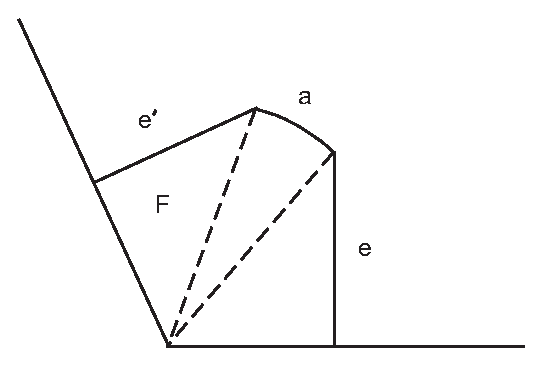
\includegraphics{PS/diag-face.eps}
  \caption{A planar region.}
  \label{fig:face}
\end{figure}

{\bf Case 1. Circumradius of $S$ is less than $\sqrt2$:}  We show
that this case does not occur.  If none of the edges of this
simplex pass through a barrier, then this simplex belongs to
$\CalQ_0'$, a case already considered.  By definition of the
wedges, the edges $\{0,v\}$, $\{0,w\}$, $\{0,w'\}$, $\{v,w\}$, and
$\{v,w'\}$ do not pass through a barrier.  Since five of the six
edges do not pass through a barrier, and since $S$ is formed by
consecutive triangles in the fan around $\{0,v\}$, the sixth does
not pass through a barrier either, by Lemma~\ref{lemma:sixth}.

%This leaves $\{w,w'\}$, which must pass through a barrier
%$T=\{u,u',u''\}$.

%No edge of the barrier $T$ can be $\{0,v\}$ because then $T$ would
%be a triangle in the fan between $w$ and $w'$, which are assumed
%to be consecutive.  No edge of $T$ can pass through a face of $S$
%because its circumradius is less than $\sqrt2$ and
%Lemma~\ref{lemma:no-pass-sqrt2}.  No other edge of $S$ can pass
%through $T$ by Lemma~\ref{lemma:single-enclosed}.  It is now
%apparent that $T$ cannot be placed anywhere at all.  This case
%cannot occur.


{\bf Case 2. Circumradius of $S$ at least $\sqrt2$:} Let
$r\ge\sqrt2$ be the circumradius.   We claim that the edge $e$
cannot extend beyond the wedge through the half plane through
$\{0,v,w'\}$.  In fact, the circumcenter of $\{0,v,w,w'\}$ lies on
the extension (in one direction or the other) of the segment $e$
to a point at distance $r$ from the origin.  If this circumcenter
does not lie in the wedge, then the orientation is negative along
one of the faces $\{0,v,w\}$ or $\{0,v,w'\}$. This face must have
circumradius at least $\sqrt2$, by Lemma~\ref{lemma:sqrt2-chi+},
and this forces the face to be a barrier.  If the orientation is
negative along a barrier, then the simplex $\{0,v,w,w'\}$ is a
simplex in $\CalQ_0$ (Lemmas~\ref{lemma:neg-orient-quad} and
\ref{lemma:neg-orient-tet}). This is contrary to our assumption
above that $\{0,v,w,w'\}$ is not in $\CalQ_0$.




%We observe that the arc marked on a unit sphere coming from a
%barrier is always as least as long as the radius marked on a unit
%sphere coming from a cone $C(u)$.  To see this, we note that the
%arc radius cut out on the unit sphere from the radial projection
%of $u$ to the edge of the cone $C(u)$ is
%$\arc(|u|,\sqrt2,\sqrt2)$. The arc cut out by an edge $\{u,u'\}$
%of a barrier $\{u,u',0\}$ is at least
%$\arc(|u|,\sqrt8,2)\ge\arc(|u|,\sqrt2,\sqrt2)$.  This establishes
%the observation.

These comments show that Figure~\ref{fig:face} correctly
represents the basic shape of $F$, with the understanding that the
edges $e$ and $e'$ may degenerate to a point.  By construction,
every point $x$ in the open convex hull $\{F,0\}$ of $F$ and $0$
lies in $C'(v)\subset \op{VC}(0)$. The convex hull $\{F,0\}$ is
the union of three solids, two Rogers simplices along the
triangles $\{0,v,w\}$ and $\{0,v,w'\}$ respectively, and the conic
solid given by the convex hull of the arc $a$, $v/2$ and $0$. By
Lemmas~\ref{lemma:rogers-app} and \ref{lemma:wedge}, these solids
have density at most $\doct$.

%By Lemma~\ref{lemma:sqrt2-unobstructed}, the origin is not
%obstructed at $x$.  Hence, if $x$ lies in the $V$-cell at $u\ne0$,
%then $|u-x|\le\sqrt2$ and $|x|\le\sqrt2$. This means that $x$ lies
%in the intersection of cones $C(v)\cap C(u)$.

%For there to be a nonempty intersection $\emptyset\ne C(v)\cap
%C(u)$, the circumradius of $\{0,v,u\}$ must be less than $\sqrt2$.
%We consider two cases depending on whether $u$ is some vertex
%$w_j$ (that is, part of the fan).

%Assume the vertex $u=w_j$ is part of the fan.  If $u=w$ or $u=w'$,
%then by construction, no point of $\{F,0\}$ is closer to $u$ than
%to the origin.  (Truncation along the edges $e$ and $e'$
%accomplishes this.) If $u\ne w,w'$, then the parts of $C(v)$ in
%the $V$-cell at $u$ lie in the two wedges alongside the leaf
%$\{0,v,u\}$ of the fan. Thus no such point lies in the wedge in
%question.  Lemma~\ref{lemma:V-cell-local} keeps the $V$-cell from
%leaking past one leaf of the fan to the next.

%Assume that the vertex $u$ is not part of the fan.  By
%construction, we have that the circumradius of $\{0,u,v\}$ is less
%than $\sqrt2$, so that some  edge of $\{0,u,v\}$ crosses a barrier
%$T$ .  The edge that crosses cannot be $\{0,v\}$ because it is too
%short (see Lemma~\ref{lemma:2t0-doesnt-pass-through}).  Let
%$\{u',u''\}\subset \{0,u,v\}$ be the edge passing through $T$.

%{\bf Case-3-b-i. The edge $\{u,v\}$ passes through $T$:} By
%Lemma~\ref{lemma:eta-barrier} at least one-endpoint of $\{v,u\}$
%forms a simplex in $\CalQ_0$ with the barrier, and $0$ is a vertex
%of $T$.  By the observation above, if there is intersection of
%$C(u)$ and $C(v)$, it must be in the convex hull of $T$ and
%$\{u,v\}$.

%If $|v|\le 2t_0$ and $\{T,v\}\not\in\CalQ_0$, then there is not
%overlap in this convex hull by Lemma~\ref{lemma:cone-avoidance}.
%If $\{T,v\}\in\CalQ_0$, then it follows that $\{w,w'\}\subset T$
%and this falls into Case~1, which has already been considered.
%Assume that $|v|\ge 2t_0$. By geometric considerations
%    $$|u-v| \ge \CalE(S(2,2,2,2t_0,2t_0,\sqrt8,2,2,2t_0)  >
%    2.77.$$
%Thus, the circumradius of $\eta(0,u,v)$ is at least
%$\eta(2.51,2.77,2) > \sqrt2$.  This is contrary to the hypothesis
%that $\eta(0,u,v)\le\sqrt2$.  Thus, this case does not occur.

% This means that we have one of
%the situations of Figure~\ref{fig:tricone}. In each case there is
%no overlap between $C(u)$ and $C(v)$, except possibly in points
%over a simplex in $\CalQ_0$.  We have used
%Lemma~\ref{lemma:cone-avoidance}, which separates the cones $C(u)$
%and $C(v)$ from the simplices in $\CalQ_0$. Thus no point of
%$\op{VC}(u)$ meets $\{F,0\}$.

%{\bf Case-3-b-ii. The edge $\{u,0\}$ passes through $T$:}  By
%Lemma~\ref{lemma:eta-barrier}, $v$ is a vertex of $T$, and either
%$\{0,T\}$ or $\{u,T\}$ is a simplex in the $Q$-system.

%Assume $S=\{0,T\}$ is in the $Q$-system.  If $x$ is not in the
%cone over $S$, then Lemma~\ref{lemma:V-cell-local} bounds the
%$V$-cell at $u$ away from $x$.  If $x$ lies in the cone over $S$,
%then $T=\{v,w,w'\}$, where $\{0,v,w\}$ and $\{0,v,w'\}$ are
%consecutive triangles in the flag around $\{0,v\}$.  This
%situation was treated in Case 1.

%Assume that $S=\{u,T\}$ is a simplex in the $Q$-system, and that
%$\{0,T\}$ is not a simplex in the $Q$-system.   Let $H$ be the
%convex hull of $T$, $u$ and $0$. If $x$ lies outside this convex
%hull, then $x$ cannot lie in the interior of both $B(u,\sqrt2)$
%and $B(0,\sqrt2)$. In fact, the shortest path outside $H$ from $0$
%to $u$ has length at least $\sqrt2$ along a face of $\{0,T\}$ and
%length an additional $\sqrt2$ along a face of $\{u,T\}$.

%Lemma~\ref{lemma:sqrt2-unobstructed} implies that $x$ cannot
%belong to $S$.  Assume that $x$ belongs to $H$. Then $x$ lies in
%the convex hull of $\{0,T\}$.  The vertex $u$ is then obstructed
%at $x$ through the barrier $T$.  Thus $x$ does not lie in the
%$V$-cell at $u$.

%This completes the proof of the claim: all points $x$ in the open
%convex hull $\{F,0\}$ of $F$ and $0$ lie in the $V$-cell at $0$.
%To complete the proof, we show that this convex hull has density
%at most $\doct$.



This completes the proof that $\sigma_R(D)$ is never positive on
non-triangular standard regions $R$.  Note that the decomposition
into the parts of cones $C'(v)$ inside a wedge is compatible with
the partition of the unit sphere into standard regions, so that
the estimate holds over each standard region, and not just over
the union of the standard regions.
%
\end{proof}






\begin{lemma}  If $R$ is a standard region that is not a triangle,
and if $\sigma_R(D)=0$, then $(R,D)$ is a quad cluster.  Moreover,
the four corners of $R$ in the quad cluster have height $2$,
forming a square of side $2$.
\end{lemma}

\begin{proof}
To analyze the case of equality, first we note that any truncation
at $1.18$ produces a strict inequality (Lemma~\ref{lemma:cone} is
strict if the volume is nonzero), so that every point must lie
over a simplex in $\CalQ_0'$ or over some $C'(v)$. We have
$\svor(S)<0$ for simplices with circumradius less than $\sqrt2$.
The only simplices in $\CalQ_0$ that produce equality are those
with five edges of length $2$ and a diagonal of length $\sqrt8$.
Any nontrivial arc $a$ produces strict inequality (see
Lemma~\ref{lemma:wedge}, so we must have that $e$ and $e'$ meet at
exactly distance $\sqrt2$ from $0$ and $v$.  Moreover, if $e$ does
not degenerate to a point, the corresponding Rogers simplex gives
strict inequality, unless $\{0,v,w\}$ is an equilateral triangle
with side length $2$.  We conclude that the entire part of the
$V$-cell over the standard region must be assembled from Rogers
simplices $R(1,\eta(2,2,2),\sqrt2)$, and quarters with lengths
$(2,2,2,2,2,\sqrt8)$.  This forces each vertex $v$ of height at
most $2t_0$ to have height $2$.  It forces each pair of triangles
$\{0,v_1,v_2\}$ $\{0,v_2,v_3\}$, that determine consecutive edges
along the boundary of the standard region to meet at right angles:
    $$\dih(0,v_2,v_1,v_3)=0.$$
This forces the object to be a quad cluster of the indicated form.
\end{proof}

We conclude the \chap\ with a proof of the main theorem.  With all
our preparations in place, the proof is short.

\begin{proof} {\bf Theorem~\ref{lemma:local-optimality} (Local
Optimality)} The hypothesis implies that there are $6$ quad clusters
and $8$ quasi-regular tetrahedra at the origin of the decomposition
star. By Lemma~\ref{lemma:1pt}, each quasi-regular tetrahedron
scores at most $1\,\pt$ with equality if and only if the tetrahedron
is regular with edge-length $2$.  By Theorem~\ref{lemma:quad0}, each
quad cluster scores at most $0$, with equality if and only if the
corners of the quad cluster form a square with edge-length $2$ at
distance $2$ from the origin. Thus, $\sigma(D)$ is at most $8\,\pt$.
In the case of equality, there are $12$ vertices at distance $2$
from the origin, forming $8$ equilateral triangles and $6$ squares
(all of edge-length $2$). These conditions are satisfied precisely
when the arrangement is $U_{fcc}$ or $U_{hcp}$ up to a Euclidean
motion.
\end{proof}
